\section{Introduction}
\label{sec:intro}

Video object removal is a fundamental task in computational photography and video
production, with applications ranging from privacy protection to cinematic post-processing.
The core challenge is twofold: (1) accurately segmenting dynamic objects across all frames,
and (2) plausibly restoring the occluded background using temporal context.

Classical approaches rely on hand-crafted optical flow and spatial inpainting
algorithms~\cite{fgvc}, which work well for simple scenes but fail on complex textures
and large occlusions. Recent advances in foundation models for segmentation---SAM~\cite{sam},
SAM~2~\cite{sam2}, Track Anything~\cite{trackanything}---and learning-based video
inpainting---ProPainter~\cite{propainter}, E2FGVI~\cite{e2fgvi}---have dramatically
improved performance, yet the interplay between mask quality and inpainting fidelity
remains underexplored.

In this work, we systematically investigate a progressive sequence of accepted
experiments:
\begin{itemize}
  \item \textbf{Route A}: Classical baseline (Mask R-CNN~\cite{maskrcnn} + optical flow + \texttt{cv2.inpaint}).
  \item \textbf{Route B}: SOTA pipeline (Track Anything~\cite{trackanything} + ProPainter~\cite{propainter}).
  \item \textbf{Route E}: SAM~3~\cite{sam3} mask refinement on top of Route~B.
  \item \textbf{Route F}: VGGT4D~\cite{vggt4d} priors converted into prompt anchors and propagated by SAM~2, the alternate backend to Route~B.
  \item \textbf{Phase~6}: Route~F masks followed by SAM~3 refinement.
\end{itemize}

We additionally explore diffusion-based inpainting (Route~G,~\cite{ldm}) and
provide a detailed failure analysis. Our contributions are:
\begin{enumerate}
  \item A reproducible, modular pipeline covering classical to geometry-guided segmentation.
  \item Systematic ablation showing that geometry priors (VGGT4D) yield the largest single
        improvement over Route~B (+0.0460 MaskScore), while SAM~3 refinement provides a
        smaller complementary gain when stacked after Route~F (+0.0010).
  \item A documented failure analysis of diffusion-based inpainting in the video domain
        under fixed Route~B masks, separating inpainting effects from mask quality.
\end{enumerate}

\begin{figure*}[t]
  \centering
  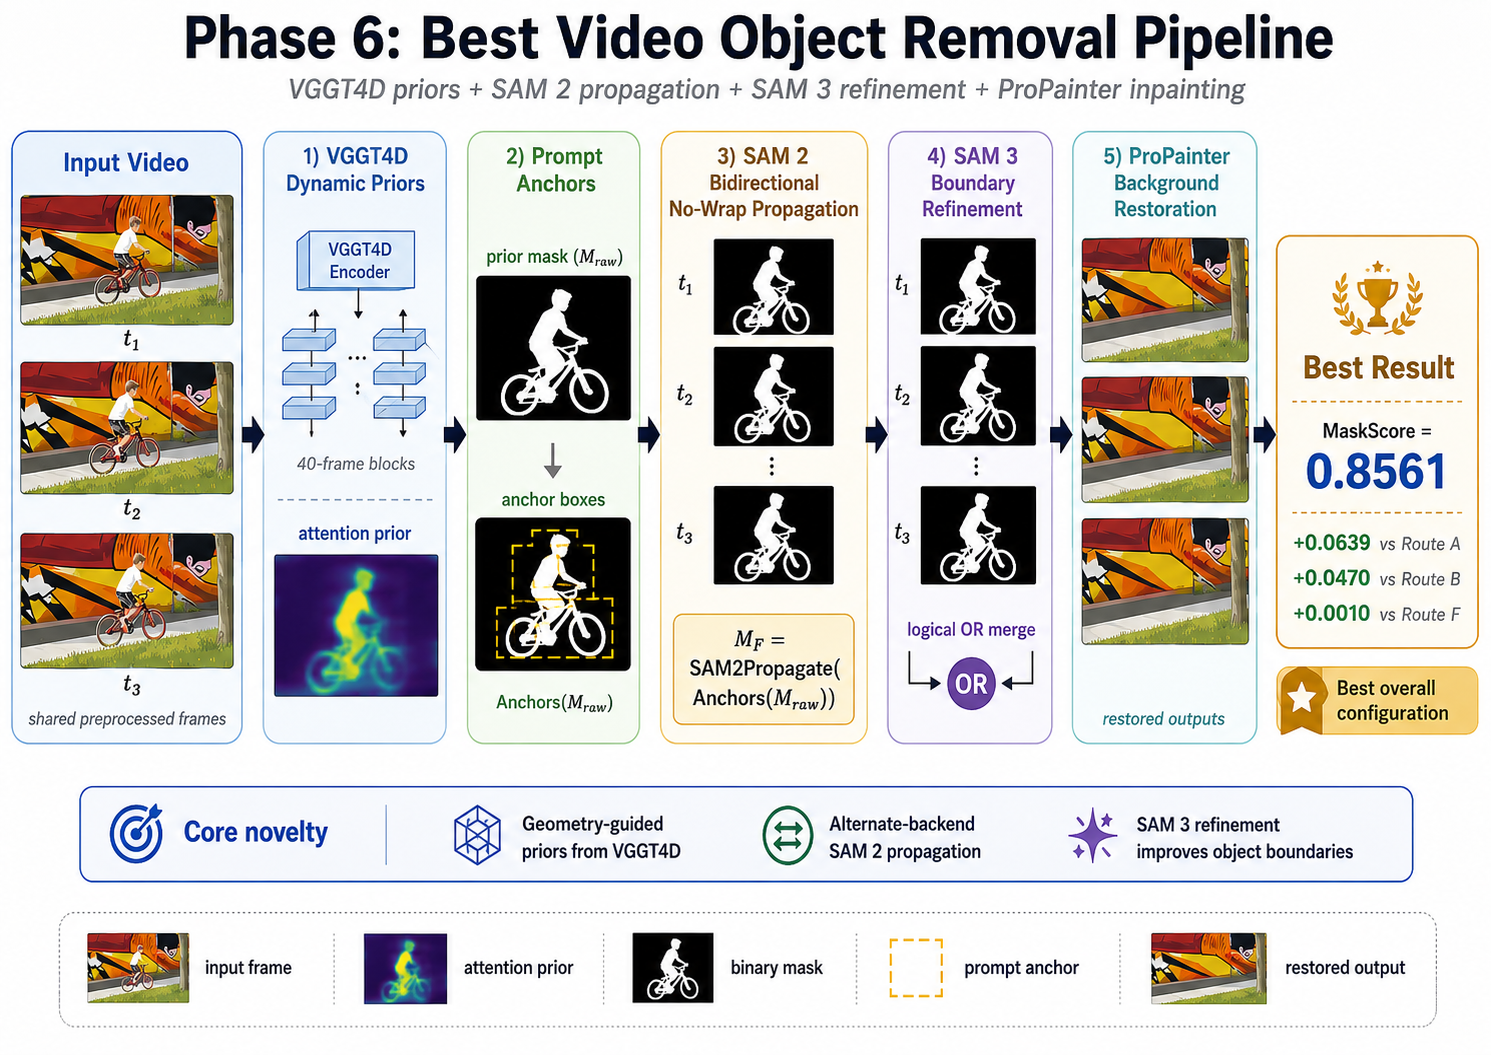
\includegraphics[width=\textwidth]{figures/fig_teaser.png}
  \caption{Teaser: visual comparison of our progressive pipeline on representative frames.}
  \label{fig:teaser}
\end{figure*}
